\documentclass[11pt,a4paper]{article}

\usepackage[utf8]{inputenc}
\usepackage[T1]{fontenc}
\usepackage{lmodern}
\usepackage[english]{babel}
\usepackage[margin=2.5cm]{geometry}
\usepackage{graphicx}
\usepackage{float}
\usepackage{booktabs}
\usepackage{tabularx}
\usepackage{longtable}
\usepackage{xcolor}
\usepackage{listings}
\usepackage{enumitem}
\usepackage{caption}
\usepackage[hidelinks]{hyperref}

\definecolor{brand}{HTML}{FF4500}
\definecolor{codebg}{HTML}{F6F7F8}
\lstset{
  basicstyle=\ttfamily\small,
  backgroundcolor=\color{codebg},
  frame=single,
  rulecolor=\color{black!15},
  breaklines=true,
  showstringspaces=false,
  keywordstyle=\color{blue!70!black},
  commentstyle=\color{black!55},
  stringstyle=\color{brand!80!black},
  columns=fullflexible,
}
\setlist{itemsep=2pt}
\graphicspath{{../images/}{../diagrams/}}
\newcolumntype{Y}{>{\raggedright\arraybackslash}X}

\title{\textbf{UAlgeddit}\\[4pt]\large A Reddit-style community platform}
\author{Web Application Development\\Martim Neves, a86010}
\date{\today}

\begin{document}
\maketitle

\begin{abstract}
UAlgeddit is a web application inspired by Reddit where users create communities (\emph{subgeddits}), publish
posts with image galleries, discuss them in threaded comments, vote on content, add friends and talk in a real-time
global chat. This report describes the requirements, the architecture of the TypeScript monorepo (a layered
Express~5 API backed by PostgreSQL through Prisma, and a React~19 single-page application styled with Tailwind CSS),
the data model, the security measures, and the engineering practices adopted: shared validation schemas, automated
tests, continuous integration, containerised deployment and internationalisation.
\end{abstract}

\tableofcontents
\newpage

% ---------------------------------------------------------------------------
\section{Introduction}

The goal of the project is a platform that makes it easy for people to share information and interact, following
the model popularised by Reddit: content is organised in topic communities, the community decides what is relevant
through votes, and discussions happen in nested comment threads.

The first version of UAlgeddit used SQLite with hand-written SQL, a flat Express structure and plain CSS. This
version is a complete re-engineering with the following goals:

\begin{itemize}
  \item a clear separation between controllers, services and repositories, organised by domain;
  \item a relational database (PostgreSQL) managed with an ORM (Prisma) and versioned migrations;
  \item a single source of truth for validation and types shared by the client and the server;
  \item Reddit-like features: multiple images per post and comment, community icons and banners, threaded replies;
  \item a modern, responsive and accessible interface with light/dark themes and three languages;
  \item robustness and security by default, automated quality checks and one-command deployment.
\end{itemize}

% ---------------------------------------------------------------------------
\section{Requirements}

\subsection{Functional requirements}

\begin{longtable}{@{}lp{13cm}@{}}
\toprule
\textbf{ID} & \textbf{Description} \\
\midrule
\endhead
FR-01 & A visitor can register (username and password) and is signed in automatically. \\
FR-02 & A user can sign in and sign out; signing out revokes every active session. \\
FR-03 & Every account has a public profile with avatar, biography, birthday, karma, posts and friends count. \\
FR-04 & A user can edit their profile and upload or remove an avatar. \\
FR-05 & A user can create a community with a unique name, a description, an icon and a banner. \\
FR-06 & The owner of a community can edit its description, icon and banner, or delete it. \\
FR-07 & Anyone can list and search communities. \\
FR-08 & A user can create a post in a community with a title, an optional body and up to ten images. \\
FR-09 & The author of a post can edit its title and body or delete it. \\
FR-10 & Anyone can browse a feed of posts from every community, a community or a user, sorted by \emph{Hot}, \emph{New} or \emph{Top}, and search posts by text. \\
FR-11 & A user can up-vote, down-vote or remove their vote on posts and comments. \\
FR-12 & A user's karma equals the sum of the scores (up-votes minus down-votes) of their posts and comments. \\
FR-13 & A user can comment on a post or reply to a comment, with text and up to four images. \\
FR-14 & The author of a comment can delete it; replies remain visible. \\
FR-15 & Comments are displayed as a collapsible tree sorted by \emph{Top}, \emph{New} or \emph{Old}. \\
FR-16 & A user can send, accept, decline and cancel friend requests, and unfriend users. \\
FR-17 & Signed-in users can talk in a real-time global chat that shows recent history and who is online. \\
FR-18 & The interface is available in English, Portuguese and French and detects the browser language. \\
FR-19 & The interface offers light and dark themes with an animated transition. \\
\bottomrule
\caption{Functional requirements}
\end{longtable}

\subsection{Quality requirements}

\begin{longtable}{@{}lp{13cm}@{}}
\toprule
\textbf{ID} & \textbf{Description} \\
\midrule
QR-01 & The interface is intuitive, responsive (phone to desktop) and accessible (keyboard, screen readers). \\
QR-02 & Credentials and sessions are protected against XSS, CSRF, brute force and user enumeration. \\
QR-03 & Every input is validated on the server; the client validates with the same rules for fast feedback. \\
QR-04 & The code is covered by automated tests executed in continuous integration. \\
QR-05 & The application can be started with a single command, starting from a clean database. \\
\bottomrule
\caption{Quality requirements}
\end{longtable}

\subsection{Constraints}

\begin{longtable}{@{}lp{13cm}@{}}
\toprule
\textbf{ID} & \textbf{Description} \\
\midrule
C-01 & The whole application is written in TypeScript. \\
C-02 & The backend uses the Express framework. \\
C-03 & The frontend uses the React library. \\
C-04 & Data is stored in a relational database (PostgreSQL). \\
\bottomrule
\caption{Constraints}
\end{longtable}

% ---------------------------------------------------------------------------
\section{Architecture}

\subsection{Monorepo}

The project is an npm-workspaces monorepo with three packages:

\begin{description}
  \item[\texttt{apps/api}] REST and WebSocket API: Express~5, Prisma, PostgreSQL, \texttt{ws}, pino.
  \item[\texttt{apps/web}] Single-page application: React~19, Vite, Tailwind CSS~4, TanStack Query, i18next.
  \item[\texttt{packages/shared}] Zod schemas, DTO types and constants imported by both applications.
\end{description}

Because the request schemas live in the shared package, a rule such as ``a title has between 1 and 300
characters'' is written once and enforced identically by the form in the browser and by the API.

In production, an nginx container serves the static bundle and reverse-proxies \texttt{/api}, the chat WebSocket
and \texttt{/uploads} to the API, so the browser only ever talks to a single origin.

\subsection{Backend layers}

Every domain (\texttt{auth}, \texttt{users}, \texttt{subgeddits}, \texttt{posts}, \texttt{comments},
\texttt{friends}, \texttt{chat}, \texttt{storage}) has its own folder with four layers:

\begin{description}
  \item[Routes] map HTTP verbs and paths to controller methods and attach middleware (authentication, uploads).
  \item[Controllers] parse parameters, query and body with the shared schemas and shape the HTTP response.
  \item[Services] hold the business rules (ownership, limits, state transitions) and throw typed errors.
  \item[Repositories] encapsulate Prisma queries and database transactions.
\end{description}

A composition root (\texttt{container.ts}) instantiates the concrete classes and injects repositories into services
and services into controllers. Services depend only on their constructor arguments, which makes them easy to test
with mocks.

\begin{lstlisting}[language=Java,caption={Composition root (excerpt)}]
const repositories = { users: new UsersRepository(db), posts: new PostsRepository(db), ... };
const services = {
  posts: new PostsService(repositories.posts, repositories.subgeddits, storage),
  ...
};
const controllers = { posts: new PostsController(services.posts), ... };
\end{lstlisting}

Errors are centralised: services throw subclasses of \texttt{AppError} (\texttt{NotFoundError},
\texttt{ForbiddenError}, \ldots) and a single error handler converts them, as well as Zod, Prisma, Multer and
body-parser errors, into a uniform JSON body. Unexpected errors are logged and answered with a generic 500.

% ---------------------------------------------------------------------------
\section{Database}

\subsection{Entity relationship model}

Figure~\ref{fig:erd} shows the entity relationship model, drawn with draw.io in crow's foot notation.

\begin{figure}[!htbp]
  \centering
  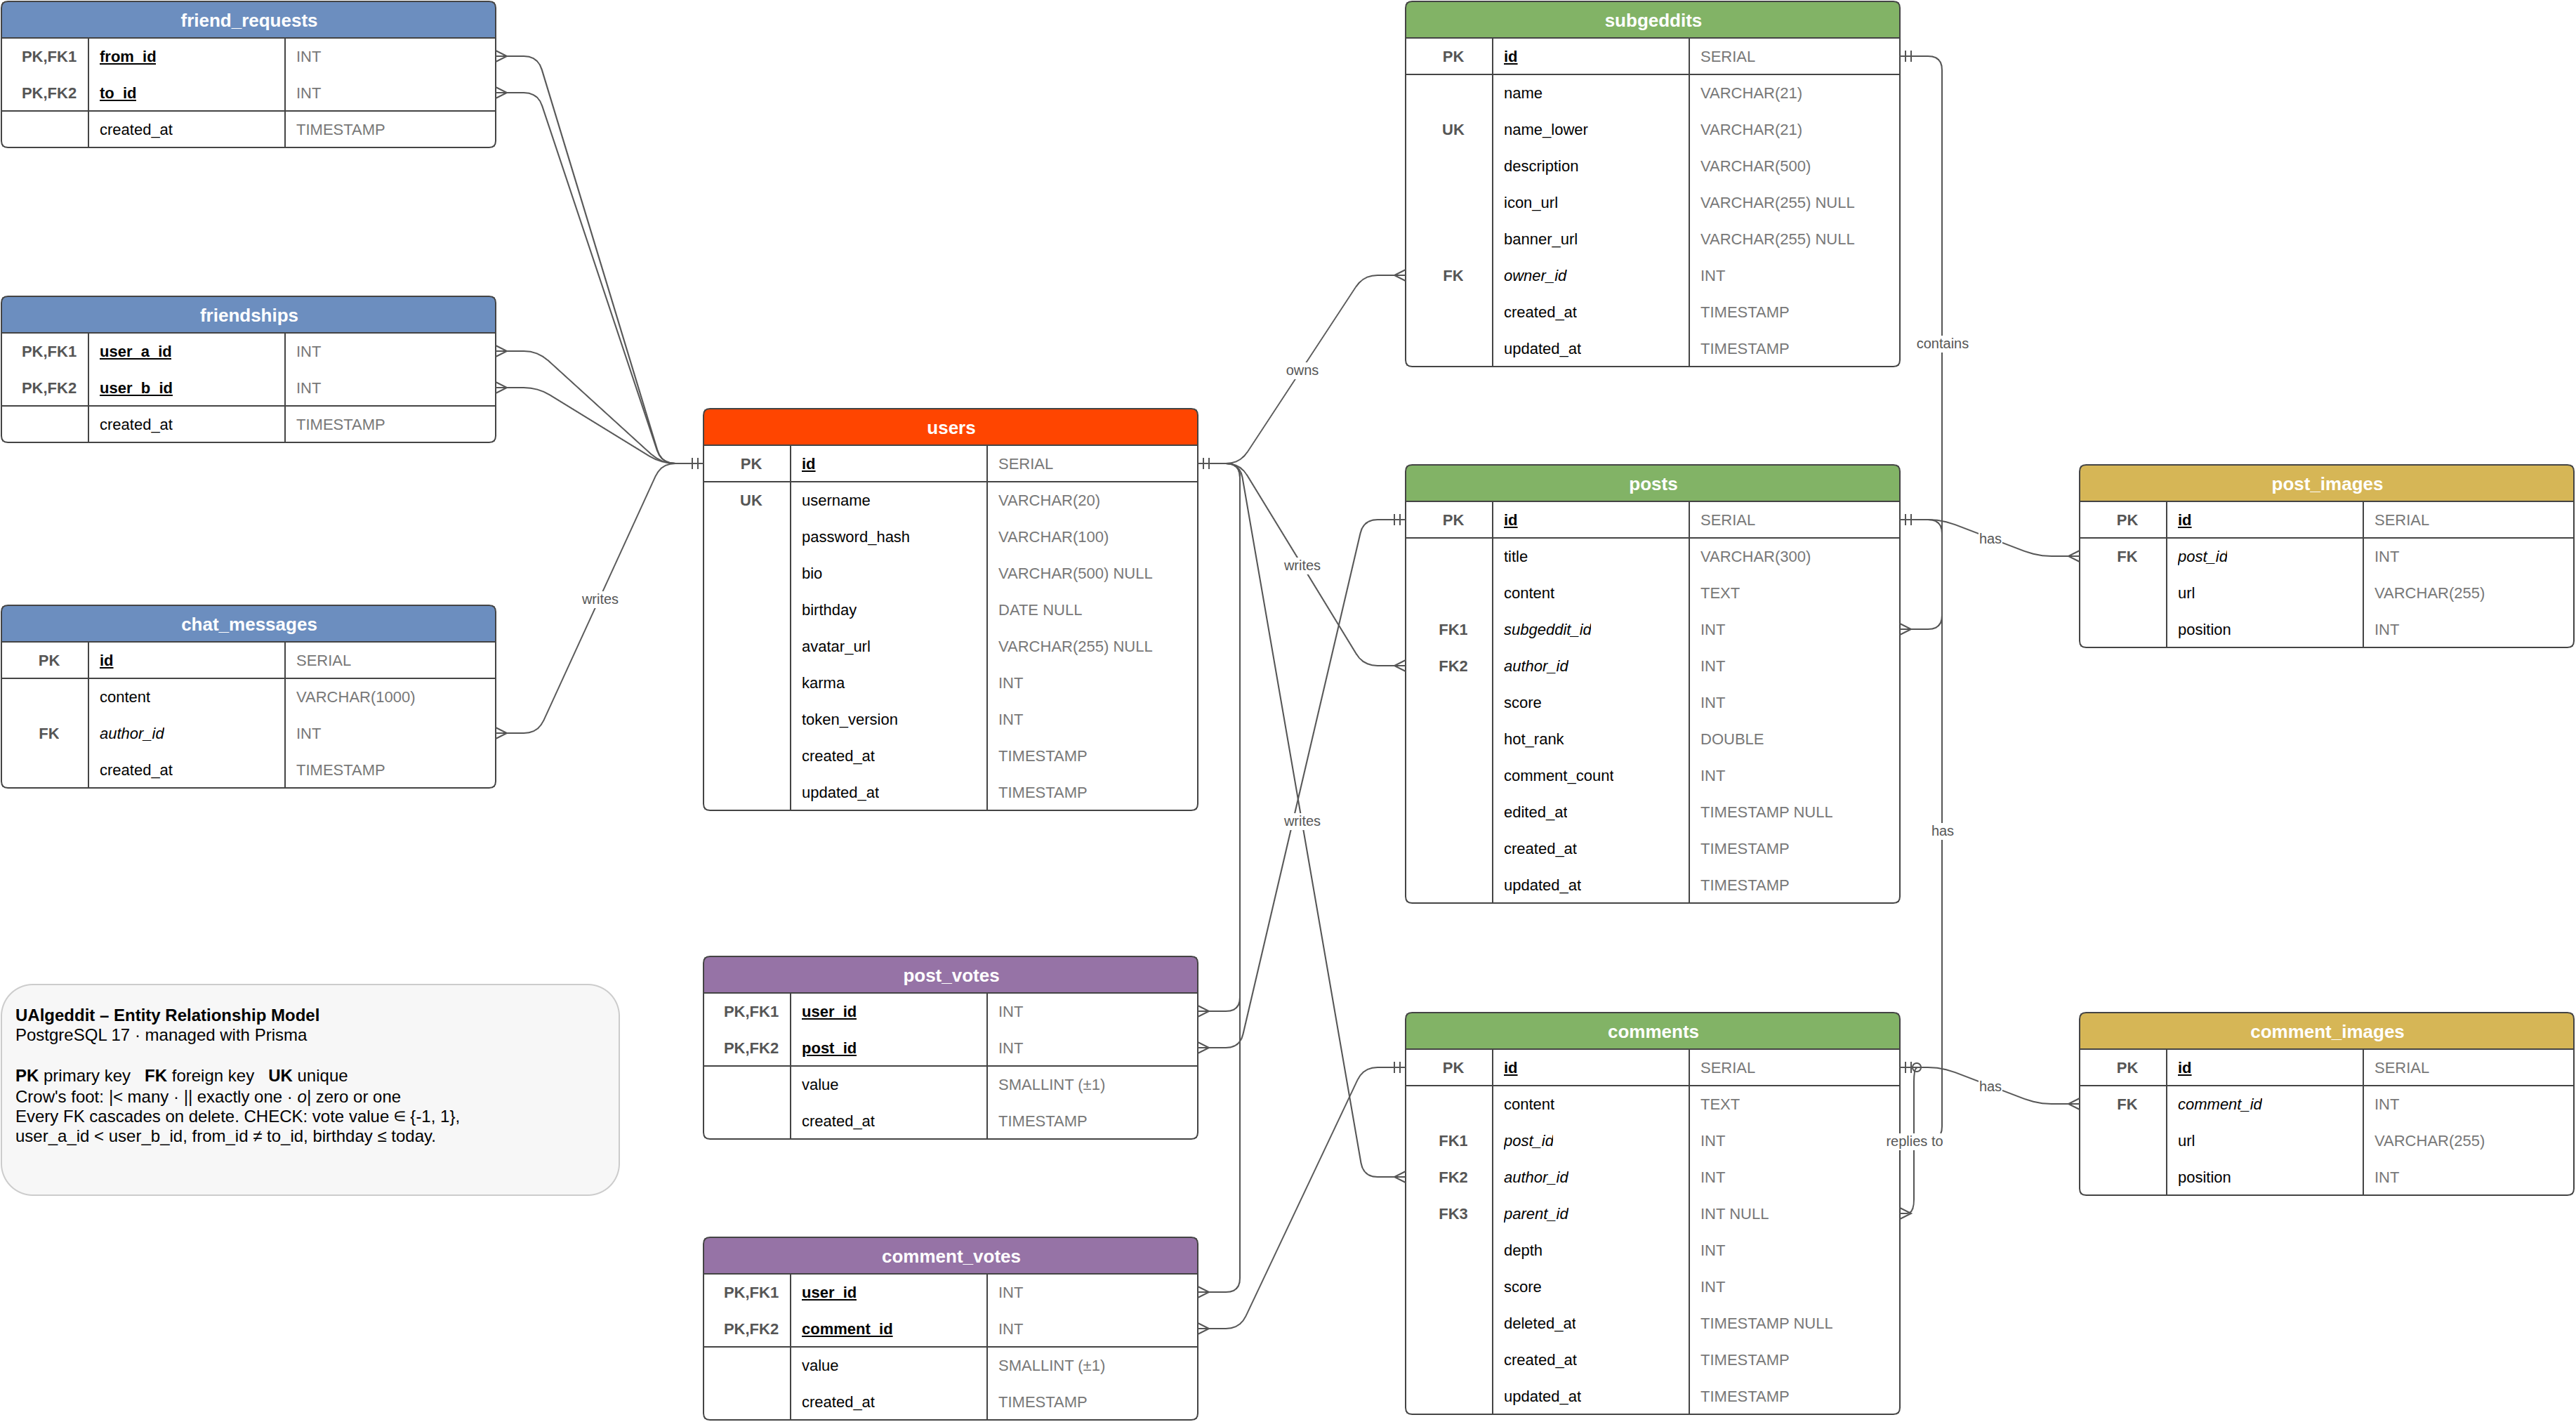
\includegraphics[width=\textwidth]{er-diagram.png}
  \caption{Entity relationship model}
  \label{fig:erd}
\end{figure}

\subsection{Relational model}

\begin{lstlisting}
users(id, username, password_hash, bio, birthday, avatar_url, karma, token_version, created_at, updated_at)
subgeddits(id, name, name_lower, description, icon_url, banner_url, owner_id -> users, ...)
posts(id, title, content, subgeddit_id -> subgeddits, author_id -> users,
      score, hot_rank, comment_count, edited_at, created_at, updated_at)
post_images(id, post_id -> posts, url, position)
comments(id, content, post_id -> posts, author_id -> users, parent_id -> comments,
         depth, score, deleted_at, created_at, updated_at)
comment_images(id, comment_id -> comments, url, position)
post_votes(user_id -> users, post_id -> posts, value)          PK(user_id, post_id)
comment_votes(user_id -> users, comment_id -> comments, value) PK(user_id, comment_id)
friend_requests(from_id -> users, to_id -> users)              PK(from_id, to_id)
friendships(user_a_id -> users, user_b_id -> users)            PK(user_a_id, user_b_id)
chat_messages(id, content, author_id -> users, created_at)
\end{lstlisting}

\subsection{Integrity rules and design decisions}

\begin{itemize}
  \item \texttt{CHECK} constraints guarantee that a vote is $+1$ or $-1$, that friendships are stored once in
        canonical order ($user\_a\_id < user\_b\_id$), that nobody befriends themselves and that birthdays are not
        in the future. Foreign keys cascade on delete.
  \item Scores, the hot rank, comment counts and karma are \emph{denormalised} and updated inside the same
        transaction as the vote or comment that changes them, so feeds are sorted and paginated with indexes.
  \item The \emph{hot} rank follows Reddit's formula
        $\mathrm{sign}(s)\log_{10}\max(|s|,1) + \frac{t - t_0}{45000}$, where $s$ is the score and $t$ the
        creation time in seconds.
  \item Comments are soft-deleted (\texttt{deleted\_at}) so reply threads keep their structure.
  \item \texttt{token\_version} allows every session of a user to be revoked without a blacklist table.
  \item Schema changes are versioned Prisma migrations; CI checks that migrations and schema never diverge.
\end{itemize}

% ---------------------------------------------------------------------------
\section{Backend}

\subsection{API}

The API is documented with OpenAPI~3.1 and served through Swagger UI at \texttt{/api/docs}. Request schemas are
generated from the shared Zod schemas, so the documentation cannot drift from the validation code.
Table~\ref{tab:api} summarises the main resources.

\begin{table}[H]
\centering
\begin{tabularx}{\textwidth}{@{}lY@{}}
\toprule
\textbf{Resource} & \textbf{Endpoints} \\
\midrule
Auth & \texttt{POST /auth/register}, \texttt{/auth/login}, \texttt{/auth/logout}, \texttt{GET /auth/me} \\
Users & \texttt{GET /users/\{username\}}, \texttt{PATCH /users/me}, \texttt{PUT|DELETE /users/me/avatar} \\
Subgeddits & \texttt{GET|POST /subgeddits}, \texttt{GET|PATCH|DELETE /subgeddits/\{name\}} \\
Posts & \texttt{GET|POST /posts}, \texttt{GET|PATCH|DELETE /posts/\{id\}}, \texttt{PUT /posts/\{id\}/vote} \\
Comments & \texttt{GET|POST /posts/\{id\}/comments}, \texttt{DELETE /comments/\{id\}}, \texttt{PUT /comments/\{id\}/vote} \\
Friends & \texttt{GET /friends}, \texttt{GET|POST /friends/requests}, accept, decline, cancel, unfriend \\
Chat & \texttt{GET /chat/messages}, WebSocket \texttt{/api/chat/ws} \\
\bottomrule
\end{tabularx}
\caption{API resources}
\label{tab:api}
\end{table}

\subsection{Authentication and security}

\begin{itemize}
  \item Passwords are hashed with bcrypt (cost 12). Login always performs a hash comparison and returns the same
        error for unknown users and wrong passwords, preventing user enumeration.
  \item Sessions are JWTs stored exclusively in an \texttt{httpOnly}, \texttt{SameSite=Lax} cookie
        (\texttt{Secure} under HTTPS). The token is never sent in a response body and \texttt{Authorization}
        headers are ignored, so scripts can never read it.
  \item State-changing requests from origins outside the allow-list are rejected (CSRF defence in depth), CORS
        only allows configured origins, and \texttt{helmet} sets security headers.
  \item Rate limits protect the whole API, the authentication endpoints and the chat.
  \item The configuration is validated at start-up; the API refuses to start with a weak secret.
\end{itemize}

\subsection{Image uploads}

Uploads are received in memory by Multer with limits on size (5~MiB), count and MIME type. The storage service
then detects the real format from the file's magic bytes (JPEG, PNG, GIF, WebP), rejecting disguised SVG or HTML,
stores the files under random UUID names and returns their public URLs. Saving is all-or-nothing, and if the
database insert fails the stored files are removed. Images are served with a sandboxing Content Security Policy.

\subsection{Real-time chat}

The chat gateway handles WebSocket upgrades on \texttt{/api/chat/ws}. It verifies the origin and the session cookie,
validates every message with the shared schema, limits each connection to five messages per five seconds,
persists messages, broadcasts them with the number of online users, and pings clients to discard dead connections.

% ---------------------------------------------------------------------------
\section{Frontend}

The client is organised by feature (\texttt{auth}, \texttt{posts}, \texttt{comments}, \texttt{subgeddits},
\texttt{users}, \texttt{friends}, \texttt{chat}). Each feature has an API module, TanStack Query hooks and its
pages and components. Server state is cached and invalidated by TanStack Query; votes are applied optimistically
to every cached copy of a post.

\begin{itemize}
  \item \textbf{Design}: Tailwind CSS~4 with semantic tokens for light and dark themes. The theme switch is
        animated with a circular reveal (View Transitions API) and respects \texttt{prefers-reduced-motion}.
  \item \textbf{Responsiveness}: a three-column layout on desktop (navigation, feed, sidebar) collapses into a
        single column with a navigation drawer on phones.
  \item \textbf{Images}: posts show a carousel with arrows, dots, a counter and a full-screen lightbox; the
        picker supports drag and drop, previews, reordering and client-side validation.
  \item \textbf{Forms}: react-hook-form with the shared Zod schemas; server validation errors are mapped back
        onto the corresponding fields.
  \item \textbf{Internationalisation}: i18next detects the browser language (Portuguese, French or English
        fallback) and remembers manual choices; dates and numbers are formatted with the active locale.
  \item \textbf{Performance}: route-level code splitting and long-term cacheable vendor chunks.
\end{itemize}

\begin{figure}[H]
  \centering
  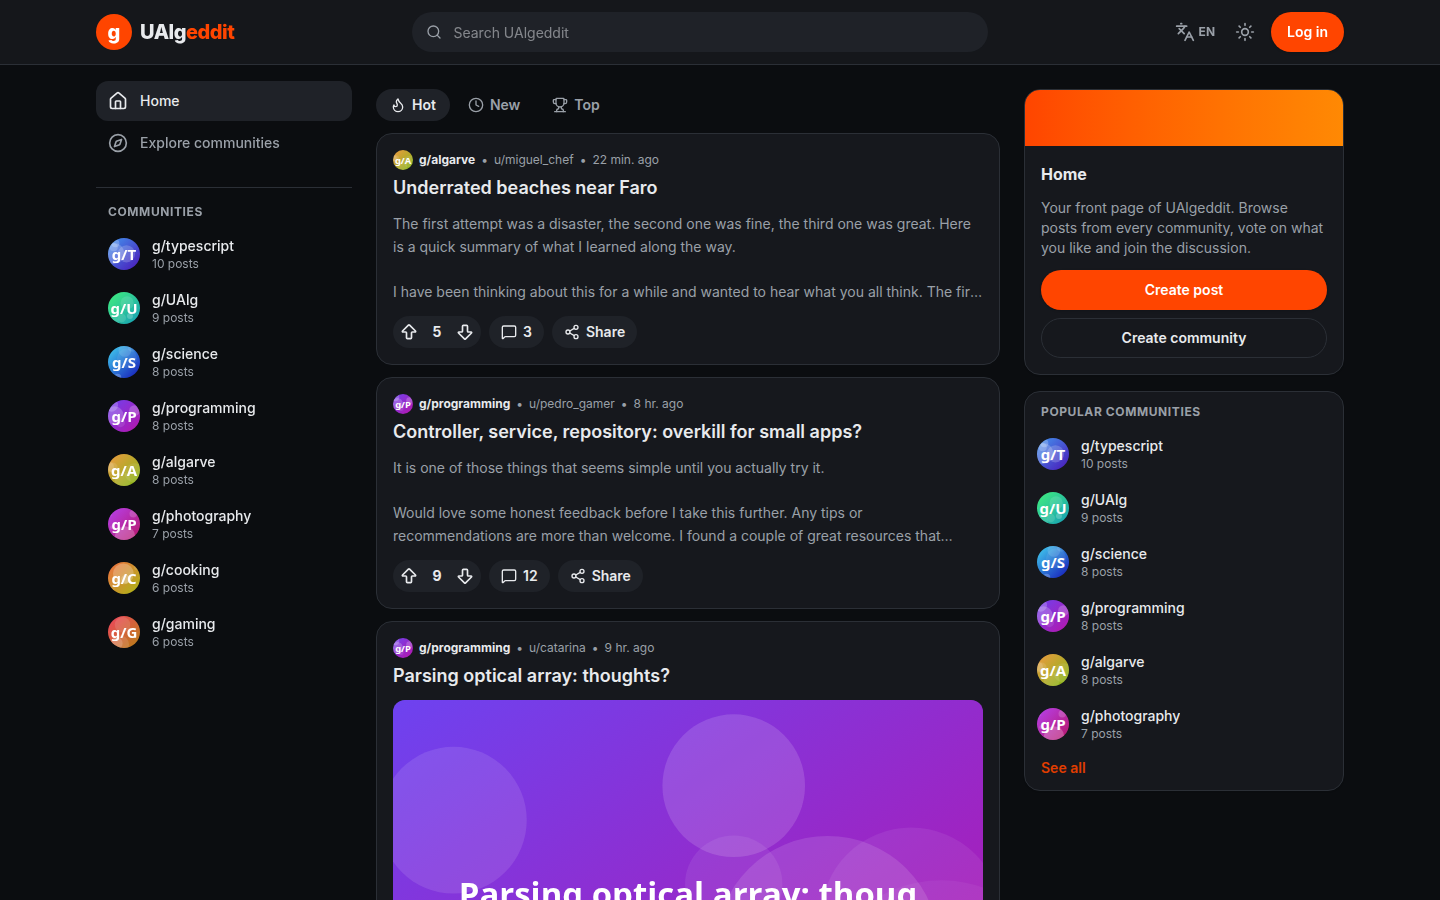
\includegraphics[width=0.49\textwidth]{home-dark.png}\hfill
  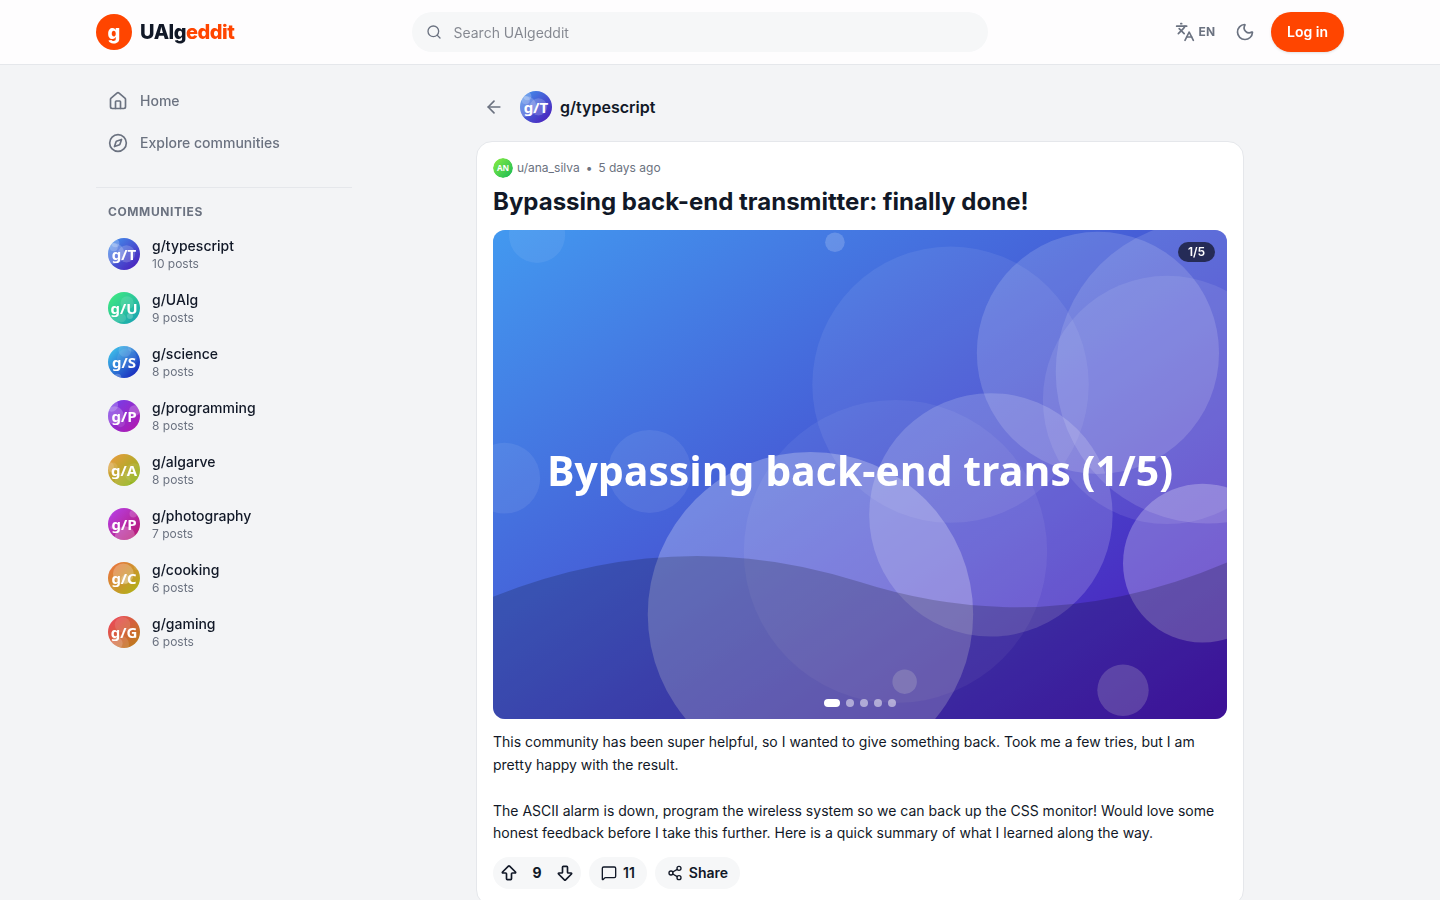
\includegraphics[width=0.49\textwidth]{post-light.png}
  \caption{Home feed (dark theme) and a post with an image gallery (light theme)}
\end{figure}

\begin{figure}[H]
  \centering
  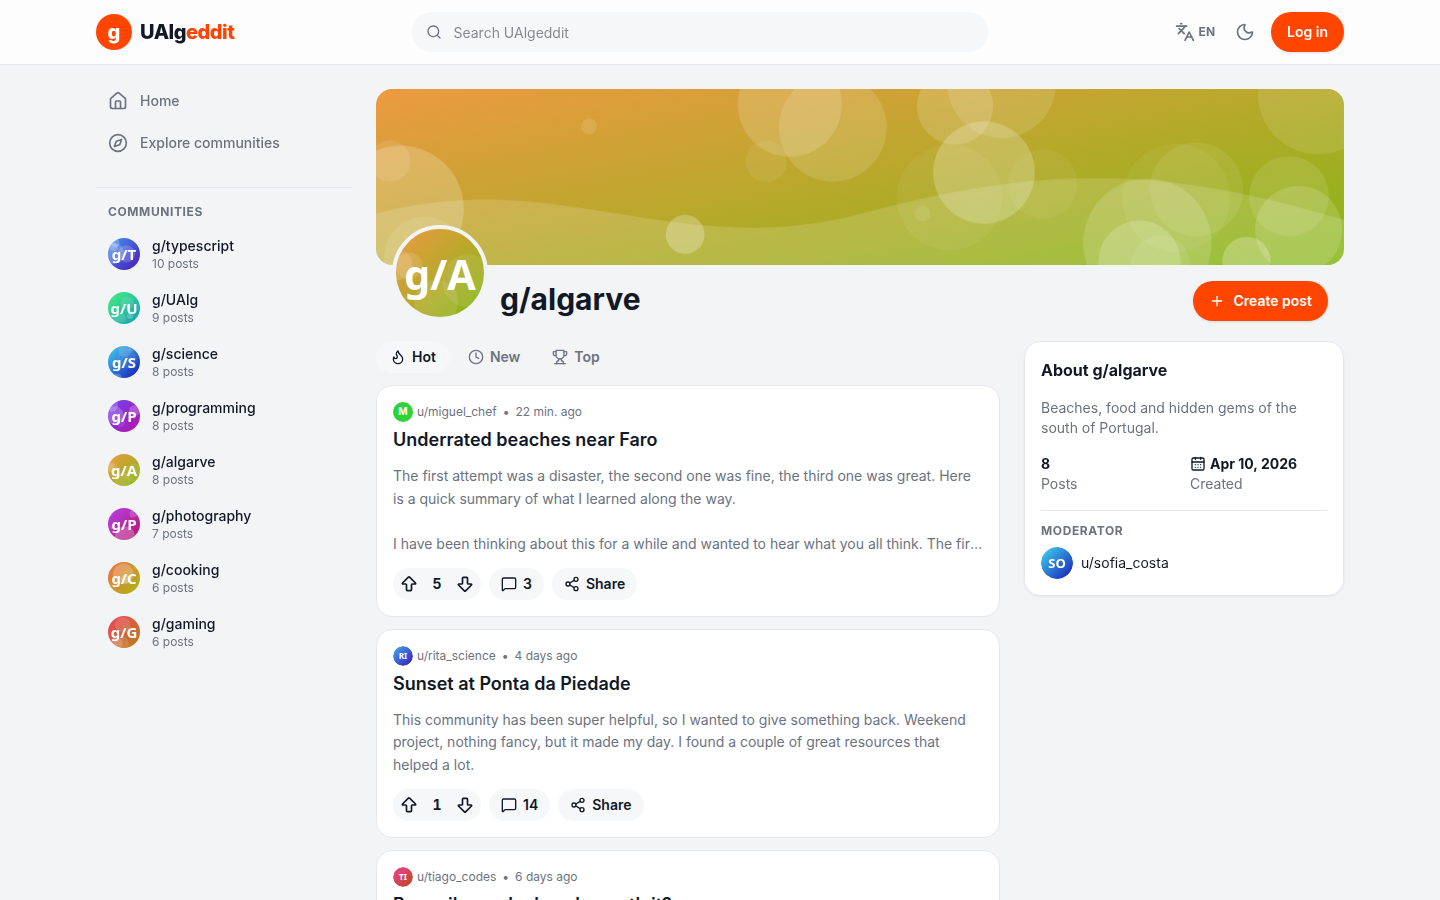
\includegraphics[width=0.62\textwidth]{community-light.png}\hfill
  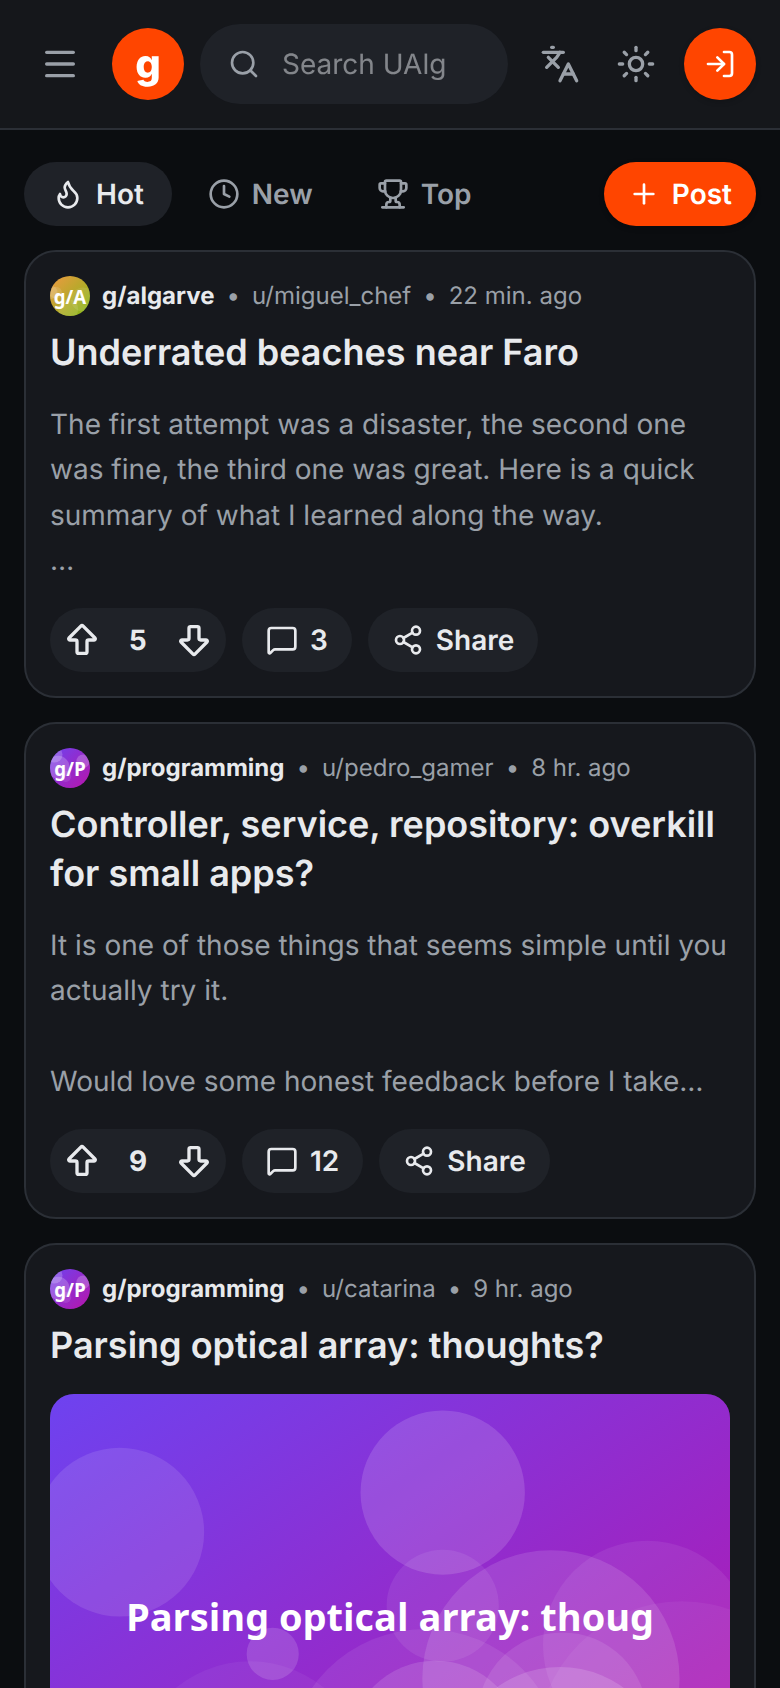
\includegraphics[width=0.22\textwidth]{mobile-dark.png}
  \caption{Community page and the mobile layout}
\end{figure}

% ---------------------------------------------------------------------------
\section{Quality and delivery}

\subsection{Testing}

Vitest runs the tests of the three workspaces. Services are unit-tested with mocked repositories, the HTTP layer
is tested with Supertest against the real Express application with stubbed services, the storage service is tested
on a temporary directory, and the client is tested with Testing Library (components, forms, utilities and the
parity of the translation catalogues).

\subsection{Continuous integration}

GitHub Actions run on every push and pull request: formatting (Prettier), linting (ESLint), type checking, unit
tests with coverage, migrations and seed against a PostgreSQL service, and the production build. A second workflow
builds the Docker images and smoke-tests the whole stack. Dependabot proposes dependency updates, and commits follow
the Conventional Commits specification.

\subsection{Deployment}

Both applications have multi-stage Docker images running as non-root users. Docker Compose starts PostgreSQL, the
API (which applies pending migrations on start-up) and nginx in order, using health checks. A Makefile wraps every
task: \texttt{make up} starts the full stack with a clean database, \texttt{make dev} starts the development
environment with hot reload, and \texttt{make ci} runs every check locally.

% ---------------------------------------------------------------------------
\section{Conclusion}

UAlgeddit evolved from a functional prototype into a maintainable, secure and well-tested application. The layered,
domain-oriented backend, the shared validation schemas and the typed data access make the code easier to reason
about and to extend, while the automated pipeline guarantees that every change is formatted, linted, type-checked,
tested and deployable. On the user side, the platform now offers the experience expected from a modern community
site: image galleries, threaded discussions, real-time chat, responsive design, themes and three languages.

Possible future work includes object storage for images, notifications, moderation tools, community
memberships and end-to-end tests.

\end{document}
